\section{MRT Module Test Unit}
\label{sec:mrt}


%Before start using \emph{MRT} testbed, its important for the user of framework to get the right understanding of MRT unit design and its role in BGPmon Test Framework.  
The \emph{MRT} unit allows one to inject MRT messages into the BGP Test Framework.  MRT messages do not come directly from a peer router. Instead they are collected by a third party and then reported to BGPmon.    An MRT message consists of a header followed by a BGP message. The header specifies the time when the message was collected and the peer that sent the message. 

% MRT messages are collected   by third parties from indirectly connected peers through third parties. 
 
The MRT unit supports two models for injecting MRT data. In the \emph{end-user} model an external user supplies the MRT data as set of files.   For example, a user may create MRT files that include BGP messages from one of her peer routers.  In the \emph{collector}
model, the tester provides a name of  RouteViews collector, a start time, and an end time.  For example, the tester may specify \emph{route-views2.oregon-ix.net}, starting from September 1st at 9:00 am, ending on September 12th at 3:00 pm. 
  
 
%  takes the fact that there are exist routing collectors that installed in Internet exchange points and collect routing data from many peers. For instance, Oregon RouteViews collectors has large number of IPv4 and IPv6 peers around the globe.   \emph{MRT} unit need to support both models no matter how fast or how often end-users or routing collectors  provide routing data to BGPmon application.  For instance, RouteViews project include more than 100 BGP peers around the world. Those peers create a very large set of updates that need to processes by BGPmon application fast and correctly. In the other hand, end-user may send small MRT file with just few BGP updates. Any MRT messages can not be dropped or ignored by BGPmon application.  

Unlike live data,  MRT files  have been collected already and each MRT message includes a time stamp. The testing  unit plays back the MRT messages, preserving the timing between messages.  For example, if the first BGP message originated at \emph{1:20:00 am} and second BGP message at \emph{1:25:00 am},  the MRT testing unit will send the first BGP message, sleep for \emph{5 minutes} and only then send the second BGP message. 

%Using \emph{timeframing} helps to create a sequence of BGP messages ordered by the time they were created at the third party.  

%Furthermore, the user of framework need to be familiar with \emph{timeframing} in MRT unit. Because MRT unit provide routing data from third parties, BGP message  timestamping plays important role in reconstructing precise routing picture on BGPmon instance. In particular, MRT format header contains  date and time  when BGP message was received at the third party. In order to replicate the right order of BGP messages, MRT unit uses the notion of \emph{timeframing}. \emph{Timeframing} is a mechanism to send BGP messages using the difference of  timestamps in subsequent BGP messages. For example, if first BGP messages originated at \emph{1:20:00 am} and second BGP messages at \emph{1:25:00 am},  MRT unit will send first BGP message and sleep for \emph{5 minutes} and only then send second BGP message. Using \emph{timeframing} helps to create a sequence of BGP messages ordered by the time they were created at the third party.  

%The  \emph{MRT}  unit is designed to achieve following goals:

%\begin{itemize}
%\item{Test BGPmon instance to receive MRT data stream.  }
%\item{Keep MRT sessions: this verifies that BGPmon is able to keep MRT %sessions alive using data from MRT stream.}
%\item{BGPmon receives routes: this verifies that BGPmon is able to extract %routes from MRT stream.}

%\item{Test BGPmon instance to scale out through chaining multiple BGPmons.   This verifies BGPmon's Chain Module functionality to create a TCP connection to another BGPmon.}
%\item{Receive XML stream: this verifies that BGPmon is able to receive XML messages from connected chain instance.}
%\end{itemize}

%\subsection{IPv4 MRT Unit Overview}

\begin{figure}
\centering
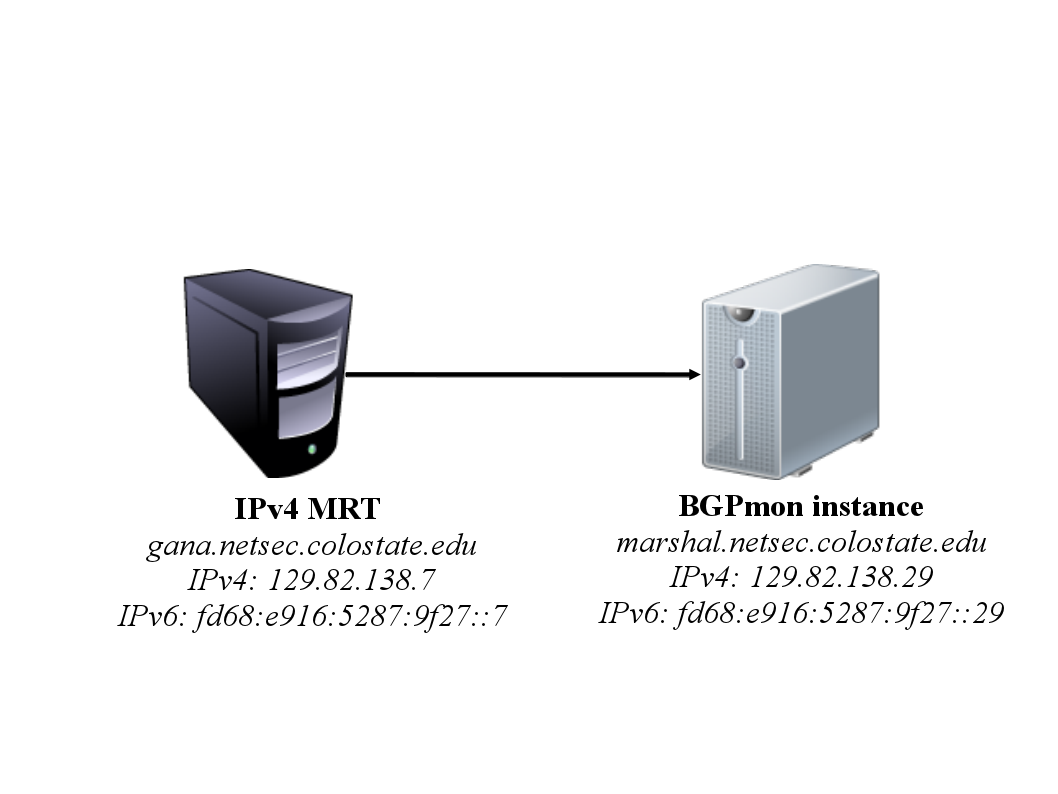
\includegraphics[scale=0.30]{figs/ipv4-mrt.png}
\caption{An overview of IPv4 MRT Unit.}
\label{mrtfig}
\end{figure}

Figure \ref{mrtfig} shows the test unit design: it includes an MRT sender and BGPmon receiver.  The  MRT sender is installed on \emph{gana.netsec.colostate.edu} with an IPv4 address of  \emph{129.82.138.7} and an IPv6 address of \emph{fd68:e916:5287:9f27::7}. The BGPmon receiver is  installed on \emph{marshal.netsec.colostate.edu} with an IPv4 address of  \emph{129.82.138.29} and IPv6 address of \emph{fd68:e916:5287:9f27::29}. 

\subsection{Configuring BGPmon to Receive MRT}
\label{sec:mrtbgpmoness}


To configure BGPmon to receive MRT data: 

\begin{enumerate}
  \item{Login to \emph{marshal.netsec.colostate.edu}}
  \item{Make sure that the BGPmon process is up and running. If not, see Section \ref{sec:essentials}.}
  \item{Telnet to \emph{localhost} port \emph{50000} to access the Command Line Interface.}
  \item{In \emph{configuration mode}, launch the \emph{mrt-listener}:}
\begin{verbatim}
marshal$ enable
marshal# configure
marshal(config)# mrt-listener enable
marshal(config)# end
\end{verbatim}      
\end{enumerate}

This command instructs BGPmon to listen for  TCP connections on \emph{marshal.netsec.colostate.edu}.   \emph{Mrt-listener } will use IPv4 address of  \emph{129.82.138.29}, port \emph{7777} and IPv6 address of \emph{fd68:e916:5287:9f27::29}, port \emph{7777} for incoming connections. 

The user of framework may configure \emph{mrt-listener} to listen for TCP connections on IPv4 address only. Run following command in \emph{configuration mode}:
\begin{verbatim}
    marshal$ enable
    marshal# configure
    marshal(config)# mrt-listener address 129.82.138.29
    marshal(config)# mrt-listener enable
    marshal(config)# end
\end{verbatim}

To configure \emph{mrt-listener} to listen for TCP connections on IPv6 address only, run:
\begin{verbatim}
    marshal$ enable
    marshal# configure
    marshal(config)# mrt-listener address fd68:e916:5287:9f27::29
    marshal(config)# mrt-listener enable
    marshal(config)# end
\end{verbatim}



%NEEDS WORK: What IP addresses are used?


%NEEDS WORK: How do we know if MRT listener is running? 
The tester of the framework can check status of    \emph{mrt-listener}. Run following command in Command Line Interface:
\begin{verbatim}
    marshal>show mrt-listener status
\end{verbatim}

This command shows \emph{mrt-listener} status. Successful configuration of  \emph{mrt-listener} will show \emph{enabled} status. Failed configuration of \emph{mrt-listener} will show \emph{disabled} status.

The tester of the framework may check the network IP addresses configured in \emph{mrt-listener}: 
\begin{verbatim}
    marshal>show mrt-listener address
\end{verbatim}

To disable the \emph{mrt-listener}  in BGPmon, run:
\begin{verbatim}
    marshal$ enable
    marshal# configure
    marshal(config)# mrt-listener disable
    marshal(config)# end
\end{verbatim}

This command instructs \emph{mrt-listener} to close TCP connections and change internal status to \emph{disabled}.



\subsection{Sending MRT Messages}

The MRT unit supports two models for injecting MRT data. In the \emph{end-user} model an external user supplies the MRT data as set of files.   In the \emph{collector} model, the tester provides a name of  RouteViews collector, a start time and an end time. 

\subsubsection{The End-user Model}

This model assumes the tester has one or more MRT files.   The tester may use his own MRT file or sample MRT file.   A sample MRT file (\emph{updates.20110916.1715})  is available on \emph{gana.netsec.colostate.edu} in the directory \emph{$\sim$bgpmoner/Development/bgpmon-dev/test/mrt\_harness/etc}.  This file was generated by \emph{route-views.oregon-ix.net} on \emph{September 16th 2011, 17:15 pm}. 

The tester of the framework need to be familiar with MRT unit directories on \emph{gana.netsec.colostate.edu}. \emph{$\sim$bgpmoner/Development/bgpmon-dev/test/mrt\_harness/etc} is directory that designed to store long-lasting files. Directory includes files that are the part of the MRT unit.  \emph{$\sim$bgpmoner/Development/bgpmon-dev/test/mrt\_harness/data} is temporary working directory. \emph{$\sim$bgpmoner/Development/bgpmon-dev/test/mrt\_harness/data}  is created to   store an optional data including  the testing MRT files. The user of the framework is allowed to store temporary files in    \emph{$\sim$bgpmoner/Development/bgpmon-dev/test/mrt\_harness/data} directory.

 
%If user chooses to use sample MRT file, he need to extract it from \emph{$\sim$bgpmoner/Development/bgpmon-dev/test/mrt\_harness/etc} and copy to  \emph{$\sim$bgpmoner/Development/bgpmon-dev/test/mrt\_harness/data}

%\begin{verbatim}
%$ cd ~bgpmoner/Development/bgpmon-dev/test/mrt\_harness/etc
%$ bunzip2  updates.20110916.1715.bz2
%$ cp updates.20110916.1715 
%               ~bgpmoner/Development/bgpmon-dev/test/mrt\_harness/data
%\end{verbatim}

%If user chooses to use his own MRT file, he need to copy it to \emph{ %$\sim$bgpmoner/Development/bgpmon-dev/test/mrt\_harness/data}.

To start MRT unit test, run following: 

\begin{enumerate}
  \item{Download the MRT files into \emph{$\sim$bgpmoner/Development/bgpmon-dev/test/mrt\_harness/data} folder or copy sample MRT file from \emph{$\sim$bgpmoner/Development/bgpmon-dev/test/mrt\_harness/etc} directory. }
  
  \item{Login to \emph{gana.netsec.colostate.edu}.}
  \begin{enumerate}
  \item{To send MRT data from \emph{filename},  run:}
\begin{verbatim}
$ mrtfeeder -f filename -d marshal.netsec.colostate.edu
\end{verbatim}
   where:
  \begin{itemize}
  \item{\emph{filename} is MRT file name in \emph{$\sim$bgpmoner/Development/bgpmon-dev/test/mrt\_harness/data}. See Section \ref{sec:mrtfeederdesign} for the details about supported \emph{filename} extensions. } 
  \item{\emph{marshal.netsec.colostate.edu} is hostname of  BGPmon receiver. MRT feeder converts
\emph{marshal.netsec.colostate.edu} hostname to an IPv4 and an IPv6 socket address structures. MRT feeder connects to BGPmon receiver using one of socket address structures. }
  \end{itemize}  
  \item{The tester of the framework may test MRT unit over IPv4 connection. Use the IPv4 address of BGPmon receiver to run MRT feeder:   }
\begin{verbatim}
$ mrtfeeder -f filename -d 129.82.138.29
\end{verbatim} 
  \item{The tester of the framework may test MRT unit over IPv6 connection. Use the IPv6 address of BGPmon receiver to run MRT feeder:}
\begin{verbatim}
$ mrtfeeder -f filename -d fd68:e916:5287:9f27::29
\end{verbatim}    
           
  \end{enumerate}
\item{To see the results, see Section \ref{sec:mrtreport}.}
\end{enumerate} 

The MRT feeder send MRT file with MRT messages  to BGPmon receiver. As long as TCP connection is alive between MRT feeder and BGPmon receiver,  BGPmon receiver  keeps track of MRT peers and received routing data.  Once the MRT feeder reaches the last MRT message in MRT file, it will close TCP connection to BGPmon.  \emph{Mrt-listener}  will be triggered to destroy all MRT sessions and processed routes. To avoid this  situation and help the tester in debugging, the MRT feeder has an option that keeps TCP connection alive. The tester of the framework can run the MRT feeder with following option:  
  
\begin{verbatim}
        $ mrtfeeder -q -f filename -d marshal.netsec.colostate.edu
\end{verbatim}
where
\begin{itemize}
\item{\emph{-q} instructs MRT feeder to keep TCP connection alive after the last MRT message is sent to BGPmon. } 
\end{itemize}

In order to stop running MRT feeder, the tester of the framework need to type following command and  press \emph{RETURN} key on a keyboard. 
\begin{verbatim}
        exit
\end{verbatim}

This command will terminate MRT unit work. 



\subsubsection{The Collector Model}


In the collector model, the tester specifies the RouteViews collector, start time and end time.  The MRT unit injects the MRT messages from a specified RouteViews collector using adjusted time frame.
%The RouteViews collector collects the MRT messages from a directly connected peers.   
%The MRT unit is designed to send stream of consequent MRT files to BGPmon receiver.  
%The MRT unit uses MRT files from the RouteViews collector and sends MRT data directly to BGPmon application. 

The RouteViews collectors provide two types of MRT files: an MRT table file and an MRT update file.  The table MRT file is the snapshot of the MRT table messages. 
%The RouteView collector generate the MRT table file every two hours.  
The update MRT file is a  set of MRT update messages. 
%The RouteViews collectors generate the  MRT update file every 15 minutes.  
The tester of the the framework provide the time frame when the MRT unit starts sending MRT snapshot and MRT update files.  The MRT unit approximate the start time to fetch the most recent   MRT snapshot file and MRT update files.  The MRT unit sends  MRT update files in a sequence based on the specified start time and end time.   

%  The MRT unit stars sending  the MRT messages that corresponds to specified start time and it stops sending MRT messages at the specified end time.
 

% that corresponds to  the time when they originated start time and end time. 


%The RouteViews collector archiving MRT messages from directly connected peers.  The MRT unit uses archived MRT files to send an MRT data to the BGPmon receiver.   The MRT unit uses two types of MRT messages: a table MRT messages and an update MRT messages.  MRT unit provide both a table and an update MRT messages to BGPmon receiver. 

To start MRT unit test, run following: 

\begin{enumerate}
  \item{Login to \emph{gana.netsec.colostate.edu}.}
  \item{Run \emph{mrtfetcher} application with following options: }
\begin{verbatim}
$ mrtfetcher -c collector -s starttime -e endtime 
   -d marshal.netsec.colostate.edu
\end{verbatim}
  where:  
  \begin{itemize}
  \item{\emph{collector} can be  \emph{route-views.oregon-ix.net}, \emph{route-views2.routeviews.org} or other collectors. The list of existing collectors is available at \url{http://www.routeviews.org/} website.}
  \item{\emph{starttime} is a unix timestamp that specifies the start time.}
  \item{\emph{endtime} is a unix timestamp that specifies the end time.}
  \item{\emph{marshal.netsec.colostate.edu} is hostname of  BGPmon receiver. MRT feeder converts
\emph{marshal.netsec.colostate.edu} hostname to an IPv4 and an IPv6 socket address structures. MRT feeder connects to BGPmon receiver using one of socket address structures. }
  \end{itemize}
  \emph{Mrtfetcher}  will send MRT files from the collector starting at time \emph{starttime} and ending at \emph{endtime}. Section \ref{sec:mrtfetcherdesign} describes the design of \emph{mrtfetcher} application.
  \item{The tester of the framework may test MRT unit over IPv4 connection. Use the IPv4 address of BGPmon receiver::   }
\begin{verbatim}
$ mrtfetcher -c collector -s starttime -e endtime 
   -d 129.82.138.29
\end{verbatim} 
  \item{The tester of the framework may test MRT unit over IPv6 connection. Use the IPv6 address of BGPmon receiver:}
\begin{verbatim}
$ mrtfetcher -c collector -s starttime -e endtime 
   -d fd68:e916:5287:9f27::29
\end{verbatim}    
  
 \item{The tester of the framework may configure MRT fetcher to skip sending MRT table messages and send MRT update messages only:}
 \begin{verbatim}
$ mrtfetcher -u -c collector -s starttime -e endtime 
   -d marshal.netsec.colostate.edu
\end{verbatim}
where
\begin{itemize}
\item{\emph{-u} flag instructs MRT fetcher to send the MRT update messages to BGPmon.}
\end{itemize}
  
  
%  NEEDS WORK: MRT fetcher sends table first and update next. 

\item{To see the results, see Section \ref{sec:mrtreport}.}
\end{enumerate} 

BGPmon receiver receives MRT data and keeps track of MRT sessions with routing data.   
%As long as TCP connection is alive to MRT feeder,  BGPmon receiver  keeps track of MRT peers and routes.  
Once the MRT fetcher reaches the last MRT message in MRT file, the MRT fetcher will close TCP connection to BGPmon.  \emph{Mrt-listener}  will be triggered to destroy all MRT sessions and processed routes. To avoid this  situation and help the tester in debugging, the MRT fetcher has an option that keeps TCP connection alive. The tester of the framework can run the MRT fetcher with following option:  


%The MRT fetcher sends a sequence of MRT messages to BGPmon receiver. Once the MRT fetcher sent the last MRT message, it closes TCP connection to BGPmon receiver. BGPmon receiver  destroys the MRT session and removes all  received BGP messages.  The tester of the framework may find this situation is difficult to debug.  To aid in debugging,  MRT fetcher application has an option that keeps TCP session alive.    The tester of the framework can run the MRT fetcher with following option:  
\begin{verbatim}
        $ mrtfetcher -q -c collector -s starttime -e endtime 
             -d marshal.netsec.colostate.edu
\end{verbatim}
where
\begin{itemize}
\item{\emph{-q} instructs MRT fetcher to keep TCP connection alive after the last MRT message is sent to BGPmon. } 
\end{itemize}

In order to stop running MRT fetcher, the tester of the framework need to type following command and  press \emph{RETURN} key on the keyboard. 
\begin{verbatim}
        exit
\end{verbatim}

This command will terminate MRT fetch unit. 


\subsection{Result Reporting}
\label{sec:mrtreport}

The MRT unit provides a set of commands for debugging the problems in BGPmon.   

In order to verify if MRT unit successfully established a TCP connection  to BGPmon receiver, run following command in Command Line Interface on BGPmon receiver:

\begin{verbatim}
marshal>show mrt clients
\end{verbatim}

This command lists the number of active MRT senders. 

To check if BGPmon instance successfully created MRT sessions, run:
\begin{verbatim}
marshal>show mrt neighbor
\end{verbatim}

This command shows the list of established MRT sessions that were extracted from MRT messages.

To check if BGPmon instance received routing data from MRT messages, user need to use destination IP address from MRT sessions in BGPmon. For example, if  there is MRT session with \emph{12.0.1.63} IP address, run following command to see received routes:

\begin{verbatim}
marshal>show bgp routes 12.0.1.63
\end{verbatim}

This command shows a report that includes the  routing information extracted  from MRT messages for \emph{12.0.1.63} MRT session. 

\subsubsection{MRT Analyzer}

To aid in debugging,  the MRT unit also has an MRT Analyzer.  The Analyzer takes an MRT file as the input and outputs a number of statistics about the peers in MRT file.  For instance, it outputs \emph{peerlist.txt} file that contains IP addresses of peers in MRT file. MRT Analyzer uses \emph{bgpdump} tool to analyse MRT messages. It extract routes from MRT file.  For each peer Analyzer prints BGP messages in human-readable format.   For instance, for a peer with  \emph{12.0.1.63} IP address, MRT Analyzer will create \emph{12.0.1.63\_table.txt} file that includes following messages:
\begin{verbatim}
BGP4MP|09/16/11 17:29:55|A|12.0.1.63|7018|
                189.45.27.0/24|7018 3549 28654 28340|IGP
BGP4MP|09/16/11 17:29:55|A|12.0.1.63|7018|1
                86.193.99.0/24|7018 3549 28654 28340|IGP
BGP4MP|09/16/11 17:29:55|A|12.0.1.63|7018|
                189.45.24.0/24|7018 3549 28654 28340|IGP
\end{verbatim}

To run MRT Analyzer:

\begin{enumerate}
\item{Login to \emph{gana.netsec.colostate.edu}.}
\item{Run MRT Analyzer:}
\begin{verbatim}
$ mrtanalyzer -c filename 
           -d ~bgpmoner/Development/bgpmon-dev/test/mrt\_harness/data
\end{verbatim}
  where:  
  \begin{itemize}
  \item{\emph{filename} is MRT file in \emph{$\sim$bgpmoner/Development/bgpmon-dev/test/mrt\_harness/data}. }
  \item{\emph{$\sim$bgpmoner/Development/bgpmon-dev/test/mrt\_harness/data} is the output directory.}
  \end{itemize}

\end{enumerate}




\subsection{MRT Source Code}
\label{sec:mrtsource}

%NEEDS WORK: Location of source code and design of tools, how to compile it

Source code of MRT unit is located in \emph{$\sim$bgpmoner/Development/bgpmon-dev/test/mrt\_harness/data}  directory.  \emph{MRT feeder}, \emph{MRT fetcher} and \emph{MRT analyzer} source code is available in \emph{$\sim$bgpmoner/Development/bgpmon-dev/test/mrt\_harness/data/src} folder. 

If user need to reinstall MRT application on \emph{gana.netsec.colostate.edu}, run following commands:

\begin{verbatim}
$ cd ~bgpmon/Development/bgpmon-dev/test_support/mrt_harness
$ make 
$ sudo make install
\end{verbatim}

This command will install \emph{MRT feeder}, \emph{MRT fetcher} and \emph{MRT analyzer} applications into the system. 


\subsubsection{Timeframing Algorithm Design Overview.}
\label{sec:timeframing}

%\begin{figure}
%\centering
%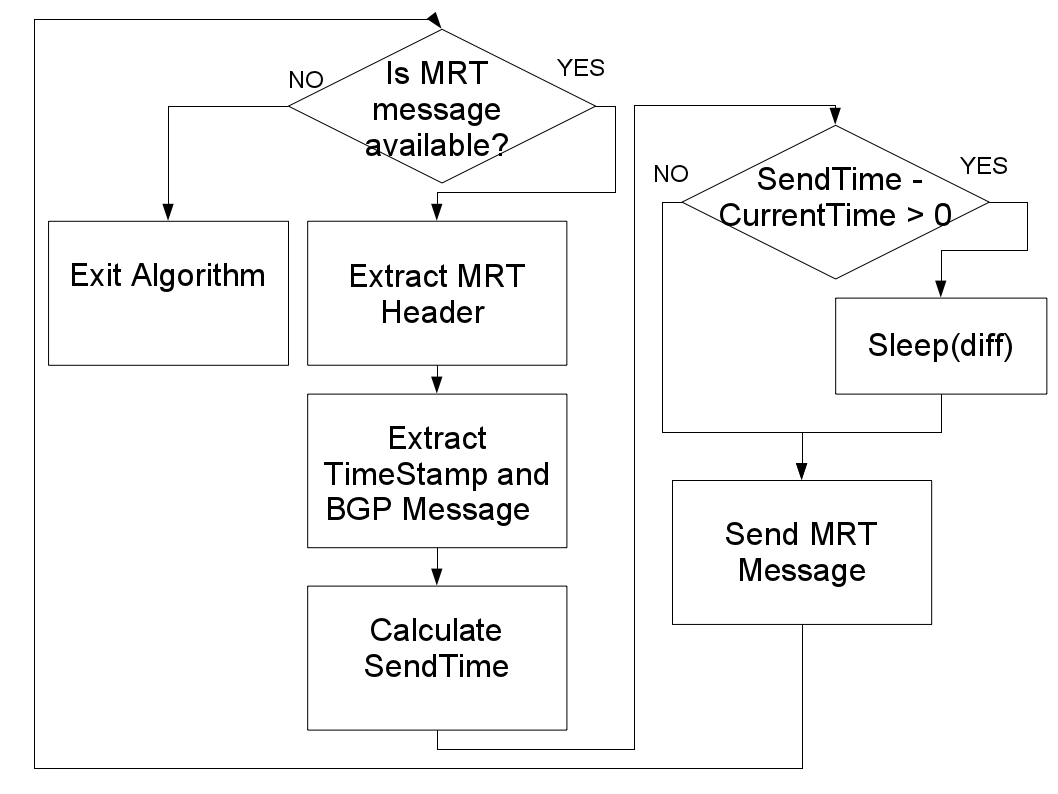
\includegraphics[scale=0.30]{figs/pacing.png}
%\caption{An overview of Timeframing Algorithm.}
%\label{pacingfig}
%\end{figure}

The MRT unit sends the MRT messages using \emph{timeframing} algorithm. Each MRT message in the MRT file has a timestamp. The timestamp in MRT header was created in the past, when the BGP message appeared at the third party.   To play the MRT messages according to the timestamp in the MRT header,  MRT unit calculates the  time shift value or,  simply, the \emph{offset}. The offset helps to adjust the time when message need to be sent. The offset is calculated as the difference in local time and the timestamp from the the first MRT message. Thus, by introducing the offset value, each MRT message requires an approximation of the \emph{sendtime}.  The sendtime indicates  the current send time of the MRT message. The sendtime is calculated as the sum of  timestamp from MRT header and the offset value.   In order to play the MRT messages at the right speed, the MRT unit compares the calculated \emph{sendtime} and the current local time. If the difference is bigger than 0, MRT unit will sleep for the difference time and only then send the MRT message.

In order to provide valid MRT data, the timeframing algorithm perform sanity check over the MRT messages. In particular, it extracts MRT header values from the MRT message and checks the data validity.  For example, a length value of BGP message in MRT header should not be bigger than the BGP message maximum size (4096 bytes). The type value in MRT header need to be equal to one from the MRT draft document.   The details of values and it's sanity check functions   are  described in the \emph{playMRT()} function design. 

The timeframing algorithm include the \emph{mrtplayer.c} and the \emph{mrtplayer.h} library files. The \emph{mrtplayer.h} is a header file that used for function declaration. The \emph{mrtplayer.c} file has source code of functions that are used in the timeframing algorithm. The \emph{mrtplayer.c} includes the  following functions: 

\begin{enumerate}


\item{\textbf{playMRT() function} }

\textbf{Definition:}  
\begin{verbatim}
int playMRT(File *p, int socket);
\end{verbatim}

\textbf{Purpose:}  playMRT() function reads the MRT file, extracts MRT messages and send them to the socket. 

\textbf{Inputs:} the MRT file descriptor, the socket file descriptor.

\textbf{Return values:}

playMRT() function has following return values: 

\begin{itemize}
\item{0: success. Function was executed successfully. }
\item{1: failure. Problem in opening the file descriptor.}
\item{2: failure. The MRT header read is less then 12 bytes.}
\item{3: failure. The MRT header read failed.}
\item{4: failure. Sanity check for timestamp value in MRT header failed}
\item{5: failure. Sanity check for type value in MRT header failed.}
\item{6: failure. Sanity check for subtype value in MRT header failed.}
\item{7: failure. Sanity check for length value in MRT header failed.}
\item{8: failure. The BGP message read is less then the length  bytes value.}
\item{9: failure. The BGP message read failed. }
\item{10: failure. Send of MRT header failed.}
\item{11: failure. Send of BGP message failed.}
\end{itemize} 

\textbf{Functionality:}

\begin{enumerate}
  \item{The playMRT() function checks if the MRT file is open. The playMRT() function check if file descriptor is not equal  to \emph{NULL}, otherwise returns 1.}
  \item{The playMRT() function reads 12 bytes of the MRT header from the file descriptor.  The MRT header is a structure that has four values: \emph{ u\_int32\_t timestamp}, \emph{u\_int16\_t type}, \emph{u\_int16\_t subtype}, \emph{u\_int32\_t length}. The  playMRT() call \emph{fread()} system function to read the data. \emph{fread()} function return the number of items successfully read. playMRT() function checks the return value:  }
  \begin{itemize}
  \item{\emph{fread} returns 12.  No problem occurred. }
  \item{\emph{fread} returns value between 1 and 11. The end of the file is reached or error occurred. The  playMRT() function returns 2.}
  \item{\emph{fread} returns 0. Error occurred. The  playMRT() function returns 3.}
  \end{itemize}

  \item{The playMRT() function performs sanity check for four values in MRT header.}
  \begin{itemize}
    \item{The playMRT() calls internal function \emph{checkTimestamp()} function.  \emph{checkTimestamp()} function takes \emph{ u\_int32\_t timestamp} in input. The  playMRT() function check the return value from \emph{checkTimestamp()} function. Return value of  0  means sanity check for timestamp succeed. If \emph{checkTimestamp()} function returns 1, sanity check failed and the  playMRT() function returns 4. }
    \item{The  playMRT() calls internal function \emph{checkType()} function.  \emph{checkType()} function takes \emph{u\_int16\_t type} in input. The  playMRT() function check the return value from \emph{checkType()} function. Return value of  0  means sanity check for type succeed. If \emph{checkType()} function returns 1, sanity check failed and the  playMRT() function returns 5. }
     \item{The  playMRT() calls internal function \emph{checkSubType()} function.  \emph{checkSubType()} function takes \emph{u\_int16\_t type} and \emph{u\_int16\_t subtype} in input. The  playMRT() function check the return value from \emph{checkSubType()} function. Return value of  0  means sanity check for subtype succeed. If \emph{checkSubType()} function returns 1, sanity check failed and The  playMRT() function returns 6. }
     \item{The  playMRT() calls internal function \emph{checkBGPlength()} function.  \emph{checkBGPlength()} function takes \emph{u\_int32\_t length} in input. The  playMRT() function check the return value from \emph{checkBGPlength()} function. Return value of  0  means sanity check for length succeed. If \emph{checkBGPlength()} function returns 1, sanity check failed and The  playMRT() function returns 7. }
  \end{itemize}
  
  \item{The  playMRT() function  calls \emph{ntohl()} system function to convert the value of length in MRT header file from  network byte order to host byte order.  }
  \item{The  playMRT() function reads \emph{N} bytes of BGP message from the file descriptor.  The \emph{N}  is the converted value of length in MRT header.   The  playMRT() calls \emph{fread()} system function to read the data. \emph{fread()} function return the number of items successfully read. The  playMRT() function checks the return value:  }
  \begin{itemize}
  \item{\emph{fread} returns \emph{N}.  No problem occurred. }
  \item{\emph{fread} returns value between 1 and \emph{N}. The end of the file is reached or error occurred. The  playMRT() function returns 8.}
  \item{\emph{fread} returns 0. Error occurred. The  playMRT() function returns 9.}
  \end{itemize}
  
  \item{The  playMRT() function  calls \emph{ntohl()} system function to convert the value of timestamp in MRT header from network byte order to host byte order. }
  \item{The  playMRT() function calculates the \emph{offset} for the timeframing algorithm. The offset is calculated as the difference of current local time and the timestamp value from  the first MRT message.  The offset value is calculated once and it never should be changed.}
  \item{The  playMRT() function calculates the \emph{sendtime} for the MRT message. The sendtime is the sum of the timestamp value in MRT header and the offset value. }\
  \item{The  playMRT() function calculates the \emph{M} value. The \emph{M} is the difference of local time and sendtime. The \emph{M} value is used to check if MRT message is ready to be sent. If the \emph{M} value is bigger than 0,  The  playMRT() uses the sleep function with \emph{M} seconds.}
  \item{The  playMRT() function uses \emph{send()} function to send  MRT header and BGP message in the socket. \emph{send()} function is called twice.  First, to send the MRT header. Second, to send the BGP message.  Upon successful completion, \emph{send()} shall return the number of bytes sent. Otherwise, -1 shall be returned. The  playMRT() function checks the return value  of \emph{send()} function:}
   \begin{itemize}
  \item{For MRT message, \emph{send()} returns 12.    No problem occurred. }
  \item{For MRT message, \emph{send()} return -1. Error occured. The  playMRT() function returns 10.}
  \item{For BGP message, \emph{send()} returns \emph{N}, where \emph{N} is the length value in MRT header. No problem occurred.}
  \item{For BGP message, \emph{send()} returns -1. Error occured.The  playMRT() function returns 11. }
  \end{itemize}
  
  \item{Upon successful sent of MRT header and BGP message, the  playMRT() function continues to read the rest of file and use the algorithm described above. The  playMRT() function extracts MRT header and BGP message until it reaches the end of the file and, in success,  it returns 0.}

\end{enumerate} % functionality

\item{\textbf{checkTimestamp() function}}

\textbf{Definition:}  
\begin{verbatim}
int checkTimestamp(u_int32_t timestamp);
\end{verbatim}

\textbf{Purpose:}  sanity check for timestamp value.  checkTimestamp() function verifies if the input  timestamp value belongs to the range of the 0 (unix time beginning) and the current unix timestamp.

\textbf{Inputs:} the timestamp value from the MRT header structure.

\textbf{Return values:}
\begin{itemize}
\item{0: success. Function was executed successfully. }
\item{1: failure. Sanity check failed.}
\end{itemize} 

\textbf{Functionality:}

\begin{enumerate}
\item{checkTimestamp() function uses \emph{ntohl()} system function to convert the timestamp value from  network byte order to host byte order.}
\item{checkTimestamp() function checks if the the converted timestamp value is bigger the 0 and less than the current time.  If timestamp value is in the range of (0;current time),  checkTimestamp() function returns 0. Otherwise, it returns 1.}
\end{enumerate}



\item{\textbf{checkType() function}}

\textbf{Definition:}  
\begin{verbatim}
int checkType(u_int16_t type);
\end{verbatim}

\textbf{Purpose:}  sanity check for type value.  checkType() function verifies if the input  type value is equal to at least one type value that defined in MRT draft document. 

\textbf{Inputs:} the type value from the MRT header structure.

\textbf{Return values:}
\begin{itemize}
\item{0: success. Function was executed successfully. }
\item{1: failure. Sanity check failed.}
\end{itemize} 

\textbf{Functionality:}

\begin{enumerate}
\item{checkType() function uses \emph{ntohs()} system function to convert the type value from  network byte order to host byte order.}
\item{checkType() function checks if the the converted type value is equal to one of the following type value:  11 (OSPFv2 type), 12  (TABLE\_DUMP type), 13 (TABLE\_DUMP\_V2 type), 16 (BGP4MP type), 17   (BGP4MP\_ET type), 32   (ISIS type), 33   (ISIS\_ET type), 48   (OSPFv3 type), 49    (OSPFv3\_ET type). In success, checkType() function returns 0. Otherwise, it returns 1.}
\end{enumerate}

\item{\textbf{checkSubType() function}}


\textbf{Definition:}  
\begin{verbatim}
int checkSubType(u_int16_t type, u_int16_t subtype);
\end{verbatim}

\textbf{Purpose:}  sanity check for subtype value.  checkSubType() function verifies if the   subtype value and the type value match to at least one category of subtype and type values  in MRT draft document. 

\textbf{Inputs:} the type value and the subtype value from the MRT header structure.

\textbf{Return values:}
\begin{itemize}
\item{0: success. Function was executed successfully. }
\item{1: failure. Sanity check failed.}
\end{itemize} 

\textbf{Functionality:}

\begin{enumerate}
\item{checkSubType() function uses \emph{ntohs()} system function to convert the type value from  network byte order to host byte order.}
\item{checkSubType() function uses \emph{ntohs()} system function to convert the subtype value from  network byte order to host byte order.}
\item{Not all types have a subtype, checkType() check specific  subtypes for the following types:  12  (TABLE\_DUMP type), 13 (TABLE\_DUMP\_V2 type), 16 (BGP4MP type), 17   (BGP4MP\_ET type).   For type  12, checkSubType() function checks if subtype if equal to 1  or 2. For type 13, checkSubType() checks if subtype is equal to 1, 2, 3, 4, 5 or 6. For type  16 or 17, checkSubType() function checks if subtype if equal  0, 1, 2, 3, 4, 5, 6 or 7.  For other types, checkSubType() does not check subtype value. In success checkSubType() return 0, in failure 1. }

\end{enumerate}




\item{\textbf{checkBGPlength() function} }

\textbf{Definition:}  
\begin{verbatim}
int checkBGPlength(u_int32_t length);
\end{verbatim}

\textbf{Purpose:}  sanity check for length value.  checkBGPlength() function verifies if the input  length value is bigger then 0 but less then the max size of BGP message (4096 bytes).

\textbf{Inputs:} the length value from the MRT header structure.

\textbf{Return values:}
\begin{itemize}
\item{0: success. Function was executed successfully. }
\item{1: failure. Sanity check failed.}
\end{itemize} 

\textbf{Functionality:}

\begin{enumerate}
\item{checkBGPlength() function uses \emph{ntohl()} system function to convert the length value from  network byte order to host byte order.}
\item{checkBGPlength() function checks if the the converted length value is bigger the 0 and less than 4096. In success, it returns 0. In failure, it returns 1.}
\end{enumerate}

\item{\textbf{MRTconnect() function} }

\textbf{Definition:}  
\begin{verbatim}
int MRTconnect(char *hostname);
\end{verbatim}

\textbf{Purpose:}  MRTconnect() function creates a socket connection to the given hostname with PORT 7777.

\textbf{Inputs:} hostname string.

\textbf{Return values:}
\begin{itemize}
\item{N:  success. Function returns a non-negative socket file descriptor.}
\item{-1: failure. The \emph{getaddrinfo()} function failed.}
\item{-2: failure. The \emph{socket} function failed.} 
\item{-3: failure. The \emph{connect} function failed.}
\end{itemize} 



\textbf{Functionality:}
  \begin{enumerate}
  \item{The MRTconnect() function identifies specified hostname. The MRTconnect() function uses the \emph{getaddrinfo()} system function. The \emph{getaddrinfo()} takes four inputs: the given hostname, the port number,   \emph{hints addrinfo} and \emph{res addrinfo} data structures. The hostname is given hostname from the input. \emph{getaddrinfo()} uses port 7777 to connect to hostname. The \emph{hints addrinfo} input points to an \emph{addrinfo} structure that specifies criteria for selecting the socket address structures  returned  in  the  list  pointed  to  by  \emph{res addrinfo}.  The MRTconnect() function checks the return value from the \emph{getaddrinfo()} function:}
  \begin{itemize}
  \item{Upon successful completion, \emph{getaddrinfo()} returns 0. }
  \item{\emph{getaddrinfo()} returns non-zero error codes that correspond to failure . The MRTconnect() function returns -1. }
  \end{itemize}
  
  \item{The MRTconnect() function uses the \emph{res addrinfo}  data structure to create a socket connection. The MRTconnect() function uses the \emph{socket()} system function to get the socket file descriptor.  The \emph{socket} function takes the \emph{ai\_family}, \emph{ai\_socktype} and \emph{ai\_protocol} values from the \emph{res addrinfo} data structure.  The MRTconnect() function checks the return value from \emph{socket()} function:  }
  \begin{itemize}
  \item{Upon  successful  completion, \emph{socket()} returns a non-negative integer (socket file descriptor.)}
  \item{In a failure, \emph{socket()} function returns -1. The MRTconnect() returns -2. }
  \end{itemize}
  
  \item{The MRTconnect() function uses \emph{connect()} function to establish a connection. The \emph{connect} function attempts to make a connection on a socket. The function takes the following arguments: the socket file descriptor, \emph{ai\_addr} and \emph{ai\_addrlen} values from 
  \emph{res addrinfo} data structure. The MRTconnect() function checks the return value from the \emph{connect} function: }
  \begin{itemize}
  \item{Upon successful completion, \emph{connect()} function return 0.}
  \item{In a a failure, -1 is returned. The main() function closes the socket file descriptor and returns -3. }
  \end{itemize}
   \item{The MRTconnect() function return the socket file descriptor.}
\end{enumerate}



\end{enumerate} %function list definition



% The Timeframing method allows to play the MRT messages at the speed they were created.  Figure \ref{pacingfig} shows the design of timeframing algorithm.  It uses MRT data files in input and  starts with repeat loop that checks if MRT messages are available. If there are no MRT messages left, algorithm exist. Otherwise, timeframing method  reads MRT messages and it extracts the MRT header with timestamp and the BGP message.   Then, it calculates the \emph{sendtime} that is used to verify if the MRT message is ready to be sent.   If the difference in \emph{sendtime - currenttime} bigger then 0, it sleeps the time difference. For example, if current time is \emph{8:00:00 am} and calculated \emph{sendtime} of MRT message is \emph{8:00:05 am}, timeframing algorithm will sleep for 5 seconds.     Once MRT message is sent to BGPmon application, the algorithm continues operate  with next available MRT message from the MRT file.  





\subsubsection{MRT Feeder Design Overview}
\label{sec:mrtfeederdesign}

The MRT feeder is an application that designed to inject MRT messages into the BGPmon Test Framework. It uses the \emph{timeframing} algorithm to send the MRT messages from the provided MRT file.  The MRT feeder application include the \emph{mrtfeeder.c} and the \emph{mrtfeeder.h} files.  The \emph{mrtfeeder.h} is a header file that used for function declarations. The \emph{mrtfeeder.c} is a source code file of MRT feeder application.  Also, the MRT feeder application includes the  \emph{mrtplayer.h} header file and use the functions defined in timeframing library. \emph{mrtplayer.c} includes the  following functions: 

\begin{enumerate}

\item{\textbf{main() function} }

\textbf{Definition:}  
\begin{verbatim}
int main(int argc, char **argv)
\end{verbatim}

\textbf{Purpose:} the main() function starts MRT feeder application. 

\textbf{Inputs:} \emph{argc} and \emph{argv} values. The argc is a count of the arguments supplied to the program and the argv is an array of pointers to the strings which are the arguments to main function. The arguments are passed to the program by the host system's command line interpreter. 

\textbf{Return values:}

The MRT feeder  uses the return values that are defined in \emph{stdlib.h} system library:
\begin{itemize}
\item{EXIT\_SUCCESS. function execution is  successful. }
\item{EXIT\_FAILURE: function execution failed.}
\end{itemize} 

\textbf{Error log printing:}

main() function uses the \emph{perror()} system function to print error messages. \emph{perror()} function produces a message on the standard error output, describing the last error encountered during a call to a system or library function.

\textbf{Functionality:}

\begin{enumerate}
  \item{The main() function starts with parsing the arguments that are provided by the user. The  main() function uses the \emph{getopt()} system function. The \emph{getopt} is design to  break  up  (parse)  options  in command lines for easy parsing by shell procedures, and to check for legal    options.  MRT feeder \emph{geptop()} function takes three inputs. First, the [-f filename] option is designed to use provided filename from the arguments.  Second, the [-d hostname] option is designed to use provided hostname from the arguments.  Third, the [-u] options is designed to set the \emph{keepTCP} integer to 1. Details of [-u] option are discussed further.  The main() function runs the while loop with true condition and checks the return value from the \emph{getopt()} function. Once the \emph{getopt} parsed the command line, it returns -1. The  main() function stops the while loop.}
  
  \item{The  main() function checks the filename extension. The user of the MRT feeder may provide archived MRT files in input. The  main() function uses the \emph{strtok()} system function. The  strtok()  function parses a string into a sequence of tokens. For a given filename, \emph{strtok()} function will lookup for a delimiter. The  main() function uses ".bz2" string as a delimiter. \emph{strtok()} inputs the filename and the delimiter and returns following values:    }
  \begin{itemize}
  \item{A NULL pointer: strtok() function could not find any token that matches the given delimiter. The  main() function will not extract the filename.}
  \item{A pointer to the last token found in filename. This means that provided filename is an archive and it need to be extracted. The main() function use \emph{system()} function to extract the filename. \emph{system()} function executes  a  command  specified  in input by calling \emph{/bin/sh -c} command. \emph{system()} function uses two inputs: the \emph{bunzip2} tool to extract the MRT file and the given filename.  The  main() function checks the return value of  \emph{system()}  function:}
  \begin{itemize}
  \item{\emph{system} function returns -1. This an error. The  main() function exits with EXIT\_FAILURE value}
   \item{\emph{system} function returns the return status of the execution of \emph{bunzip2} command. \emph{bunzip2} returns 0 for a normal exit and 1 for  environmental problems (file not found, etc.)  In case of 1,  the  main() function exits with EXIT\_FAILURE. In case or 0, filename was successfully extracted.}
  \end{itemize}  
  
  \end{itemize}

  \item{The  main() function opens the filename. The  main() function uses the \emph{fopen()} system function to open the filename. \emph{fopen()} function takes two inputs, first the given filename and second, the mode. The  main() function uses "rb" mode to open binary MRT file for a read. The  main() function checks the return value of \emph{fopen} function. }
  \begin{itemize}
  \item{\emph{fopen} function returns a NULL pointer. An error occured. The  main() function exits with EXIT\_FAILURE value.}
  \item{Upon successful completion \emph{fopen} function returns  the file descriptor. }
  \end{itemize}
  
  
  \item{The  main() function  uses the \emph{MRTconnect()} function from the \emph{mrtplayer.c} library. \emph{MRTconnect()} takes the hostname in input and returns the socket file descriptor. The main() function checks the return value from the \emph{playMRT()} function.}
   \begin{itemize}
  \item{In a success, the \emph{MRTconnect()} function returns a non-negative value (the socket file descriptor). }\
   \item{In a failure, the \emph{MRTconnect()} function returns a error number. The main() function uses the \emph{switch()} system function to print the corresponding error  message. In a failure, the main() function closes the file descriptor and exits with EXIT\_FAILURE value.}
  \end{itemize}
  
    
  \item{The  main() function  uses the \emph{playMRT()} function from the \emph{mrtplayer.c} library. The  \emph{playMRT()} function takes two inputs: the file descriptor and the socket file descriptor. The \emph{playMRT()} function send the  MRT data via socket connection. The main() function checks the return values from the \emph{playMRT()} function. The main() function checks the return value from the \emph{playMRT()} function.}
  \begin{itemize}
  \item{In a success, the \emph{playMRT()} function returns 0. }\
   \item{In a failure, the \emph{playMRT()} function returns a error number. The main() function uses the \emph{switch()} system function to print the corresponding error  message. In a failure, the main() function closes the file descriptor,  the  socket file descriptor and exits with EXIT\_FAILURE value.}
  \end{itemize}
  
  
  \item{After the the main() function sent the MRT file, it  checks the \emph{keepTCP} integer value.    The \emph{keepTCP} value is set to 1 if  the MRT fetcher application was started with \emph{-u} options at the command line. In the design of MRT feeder, this option is created to leave TCP connection open until the user types "exit" in command line. }
  \begin{itemize}
  \item{If \emph{keepTCP} is enabled, the main() uses a while loop with true condition and it uses  two functions: \emph{fgets()} and \emph{strcmp()}.  In the while loop the main()function calls \emph{fgets} to read the data from the command line.  The \emph{fgets} function has three inputs: the \emph{char buffer}, the size of the char buffer and the source of the stream.  The main() function define the char buffer \emph{buf} with size of 100 bytes. The source of the stream is \emph{stdio}.  The main() function  checks  the \emph{fgets()} function return values.}
  \begin{itemize}
  \item{On error, the \emph{fgets()} function return NULL. The main() function closes}
  \item{Upon successful completion, \emph{fgets()} returns the read characters from command line. }
  \end{itemize}
  \item{In the while loop,  the main() function use the \emph{strcmp()} function. The \emph{strcmp()} function  compares the two input strings. The first input string is string from the char buffer that \emph{fgets} provides. The second string is defined "exit" string.  The main() function checks the \emph{strcmp()} function return values.  }
  \begin{itemize}
    \item{If two strings are equal, the \emph{strcmp()} function returns 0. The main() function breaks the while loop. }
  \item{If two strings are different, the \emph{strcmp()} function returns the byte difference between two strings.  The main() function continues to loop the while loop  and reads the input from the command line.}
  \end{itemize}
  \end{itemize}
  
  \item{The main() function uses \emph{close()} function to close the file descriptor and the socket file descriptor. Lastly, the main() function will exit with EXIT\_SUCCESS value. }
  

\end{enumerate}



\end{enumerate} %function list definition


%\begin{figure}
%\centering
%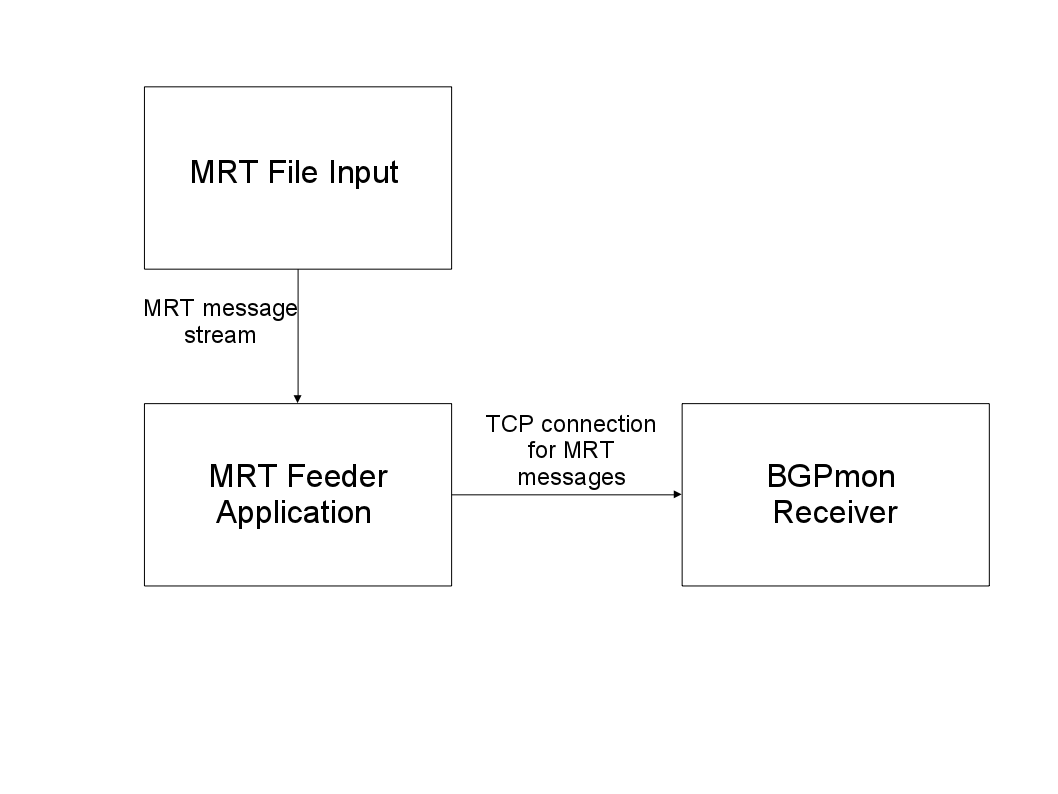
\includegraphics[scale=0.30]{figs/mrtfeeder-design.png}
%\caption{An overview of MRT Feeder application.}
%\label{feederdesignfig}
%\end{figure} 

%The MRT feeder is an application that designed to inject MRT messages into the BGPmon Test Framework.  Figure \ref{feederdesignfig} shows the design of  MRT feeder application. Figure shows the inputs and the outputs of the system.  The MRT File Input provides MRT files. In case of MRT File Input provides archived MRT files, the MRT feeder extracts the MRT file.  The BGPmon application is receiver that receives MRT messages.    The MRT feeder takes the MRT file from MRT File Input instance, extracts MRT messages and send them to BGPmon application over TCP connection.  

%\begin{figure}
%\centering
%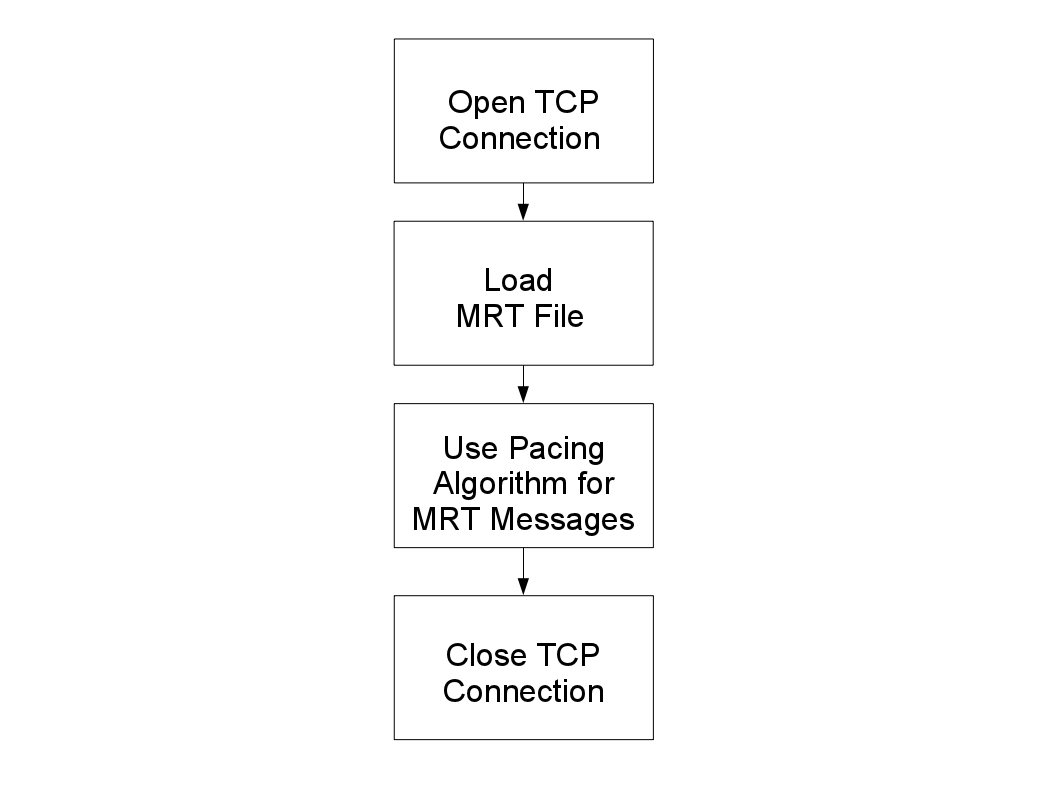
\includegraphics[scale=0.30]{figs/mrtfeeder-flow.png}
%\caption{MRT Feeder Data Flow Overview.}
%\label{feederflowfig}
%\end{figure}

%Figure \ref{feederflowfig} shows the data flow in MRT feeder. There are few simple components that are used in the MRT Feeder.   When the MRT Feeder application is executed, first it opens a TCP connection to BGPmon receiver.  Second, the MRT Feeder opens the MRT file from the input. Third, the MRT feeder uses \emph{timeframing} algorithm to extract and send MRT messages to BGPmon. \emph{Timeframing} alrotihgm is described in Section \ref{sec:timeframing}.  MRT feeder plays MRT messages at the same speed as they were received at the third party.  Once the MRT feeder reaches the end of the MRT file, it closes TCP connection to BGPmon receiver. 

%The MRT feeder has following running options:


%\begin{verbatim}
%$ mrtfeeder [-u] [-f filename] [-d host]
%\end{verbatim}
%   where:
%  \begin{itemize}
%  \item{\emph{-u} is an options that force MRT feeder to keep TCP connection when the MRT feeder %sent all MRT messages.}
%  \item{\emph{-f filename} is an MRT file name.  The user may provide archived file name. The MRT %feeder looks into the file name and detects if MRT file need to be extracted. }
%  \item{\emph{-d host} is name of the host that runs BGPmon receiver. }
%  \end{itemize}  
  
  
  
%The MRT feeder works as follows. The MRT feeder opens a single TCP connection to BGPmon receiver.  The MRT feeder takes the MRT file name and opens it to read MRT messages.  For each MRT message, the MRT feeder extracts the timestamp and the BGP message.   MRT feeder uses the \emph{timeframe} mechanism to send MRT messages.  For instance, if the first  MRT message originated at \emph{8:00:00 am} and the second MRT message at \emph{8:00:03},  MRT fetcher will send the first MRT message, wait for 3 seconds and send the second MRT message. \emph{Timeframe} mechanism allows the tester of the framework to play MRT messages at the right speed.  Once the all MRT messages from the MRT file are sent,  MRT feeder has an option (\emph{-u} flag in input)  to close TCP connection  or leave  it open until the user of the framework terminates it manually. This option helps in debugging BGPmon application.
 



\subsubsection{MRT Fetcher Design Overview}
\label{sec:mrtfetcherdesign}

%The MRT feeder application include the \emph{mrtfeeder.c} and the \emph{mrtfeeder.h} files.  The \emph{mrtfeeder.h} is a header file that used for function declarations. The \emph{mrtfeeder.c} is a source code file of MRT feeder application.  Also, the MRT feeder application includes the  \emph{mrtplayer.h} header file and use the functions defined in timeframing library. \emph{mrtplayer.c} includes the  following functions: 

The MRT fetcher application is designed to run in the \emph{collector mode}. The MRT fetcher application goal is to imitate the behaviour of the routing collector. The routing collector sends two types of data: the MRT table snapshot that provides a set of  routing tables from connected peers and sequential set of MRT update messages that update the routing information.  The  The MRT fetcher application is designed to send MRT data from the existing routing collectors.  In particular, it uses the RouteViews collector's archives to fetch the MRT data. The MRT fetcher takes two unix timestamps: the \emph{start time} and the \emph{end time}. The \emph{start time} specifies the time when MRT fetcher sends the MRT messages. The  \emph{end time} specifies the time when the MRT fetcher stops sending the MRT data.   The RouteViews collectors provides the MRT tables that are generated every two hours and the MRT update files that are generated every 15 minutes. The MRT fetcher application goal is to send the MRT data that originated between \emph{start time} and the \emph{end time}.  

The MRT fetcher is designed in following way. First,  the MRT fetcher calculates the \emph{table time}. The \emph{table time} is unix time that specifies the most recent (in the range of 2 hours) MRT table snapshot. The \emph{table time}  is calculated as the nearest integer divisible by 7200. For example, if the input \emph{start time} is equal to \emph{1317203100} (Sept 22, 2011, 9:45:00 am), the \emph{table time} is calculated as  integral part of \emph{star time} divided by 7200  and  multiplied by 7200. The calculation gives the \emph{table time} to be equal to 1317196800 (Sept, 22, 2011, 8:00:00 am) and it gives the most recent  unix time of MRT table file. The MRT fetcher downloads  the proper MRT table file from the RouteViews collector archive.   The MRT fetcher extracts the archive and use \emph{send()} function  to  send the MRT table file via socket connection.  Second,  the MRT fetcher is designed to play MRT  update messages at the right speed that corresponds to specified \emph{start time} and \emph{end time}.  In the example above, the MRT fetcher is 1 hour and 45 minutes below the requested \emph{start time}. In order to get to the MRT update messages  originated at \emph{starttime}, the MRT fetcher sends MRT update messages starting from \emph{table time} and ending the \emph{start time} values. The MRT fetcher does not apply timeframing algorithm to those messages. The MRT fetcher fetches and  sends 7 MRT update files that fall in the 1 hour and 45 minutes gap.   Third, the MRT fetcher is ready to play the messages that originated from \emph{start time} and ends on the \emph{end time}. The MRT fetcher fetches each MRT update message from the RouteViews archive and sends it using the \emph{timeframing} algorithm.

%In addition, proposed design has some number of  challenges. In particular,

%In MRT fetcher, the  fetching of MRT data from RouteViews archive takes some amount of time. Also, extracting of MRT data files takes time too. 
%In one hand, possible delays in retrieving and unzipping the data may create time gap between the MRT update files.  Every update message file from RouteView archive is a set of MRT messages. 
The \emph{timeframing} algorithm plays the messages at the right speed. This means that the set of MRT messages from the MRT update file is spread across 15 minutes interval. In the \emph{timeframing}  algorithm two or more MRT messages may have a few seconds delay. And \emph{timeframing} algorithm calculates the time time when those messages need to be send.  In MRT fetcher, fetching the MRT file and extracting the MRT file takes the time. The MRT fetcher creates a small timing gap between the two MRT files. This gap is measurable in order of few seconds and does not affect the overall speed of sending MRT files.    

 

\begin{enumerate}

\item{\textbf{main() function} }

\textbf{Definition:}  
\begin{verbatim}
int main(int argc, char **argv)
\end{verbatim}

\textbf{Purpose:} the main() function starts MRT fetcher application. 

\textbf{Inputs:} \emph{argc} and \emph{argv} values. The argc is a count of the arguments supplied to the program and the argv is an array of pointers to the strings which are the arguments to main function. The arguments are passed to the program by the host system's command line interpreter. 

\textbf{Return values:}

main() function uses the return values that are defined in \emph{stdlib.h} system library:
\begin{itemize}
\item{EXIT\_SUCCESS. function execution is  successful. }
\item{EXIT\_FAILURE: function execution failed.}
\end{itemize} 

\textbf{Error log printing:}

The main() uses the \emph{perror()} system function to print error messages. \emph{perror()} function produces a message on the standard error output, describing the last error encountered during a call to a system or library function.

\textbf{Functionality:}
NEEDS WORK: section requires a lot details.
\begin{enumerate}



\item{The main() uses the \emph{getopt()} function to parse command line. }

\item{The main() checks the RouteView collector name. Based on collector name string, the main() function chooses the right URL to fetch the MRT data.  }

\item{The main() function calls the \emph{MRTconnect()} function twice to establish two TCP connecitons. One is designed to send MRT table file, another - to send the MRT update file.}

\item{The main() function uses the starttime from the input and  calculates the \emph{table time}. }

\item{The main() uses the \emph{libcurl} library to fetch the MRT table file from the Routeview collector.  The \emph{libcurl} saves archive in \emph{/home/bgpmoner/Development/bgpmon-dev/test/mrt\_harness/data} folder. }

\item{The main() function extracts the MRT table file. }
\item{The main() function sends the MRT file using the first socket file descriptor.}
\item{The main() function closes the socket file descriptor.}

\item{The main() function uses three timestamps variables: the \emph{table timestamp}, the \emph{start time} and the \emph{end time}.  For a range of [\emph{table timestamp; start time}), the main() function fetches the corresponding  MRT update file, extract it and use \emph{send()} system function to write the data to the socket file descriptor. If [\emph{table timestamp; start time}) includes many MRT update files, the main() function will repeat the previous step until the last MRT update that falls within the range. For a range of [\emph{start time; end time}), the main() function fetches the  corresponding MRT update file, extract it and use the \emph{timeframing} algorithm to send MRT messages at the right speed.  If [\emph{ start time; end time}) includes many MRT update files, the main() function will repeat the previous step until the last MRT update that falls within the range. }

% The \emph{MRT table timestamp} is the unix timestamp of MRT table file. The \emph{starttime} and the \emph{endtime} are the unix timestampes that come from the MRT fetcher startup arguments.  The main() function use \emph{for loop} to send the MRT update files. The \emph{for loop} uses the timestamps described before.   In the \emph{for loop}, the start index starts from \emph{MRT table timestamp}, the end condition is the \emph{endtime},  the increase index is 900 seconds (15 minutes) interval between each MRT update file.    For each index in the \emph{for loop}, the main() function calculates the name of the MRT update file.  Then, it uses \emph{libcurl} to download the file.  Each downloaded file need to be extracted.     
%The \emph{for loop} has an \emph{if} statement that checks if index becomes bigger then the \emph{starttime} from the input. 




\item{For each of MRT update files, the main()  function uses the \emph{libcurl} library to fetch the MRT update  messages. }


\item{The main() function closes the socket file descriptor.}




\end{enumerate}

\end{enumerate}



%\begin{figure}
%\centering
%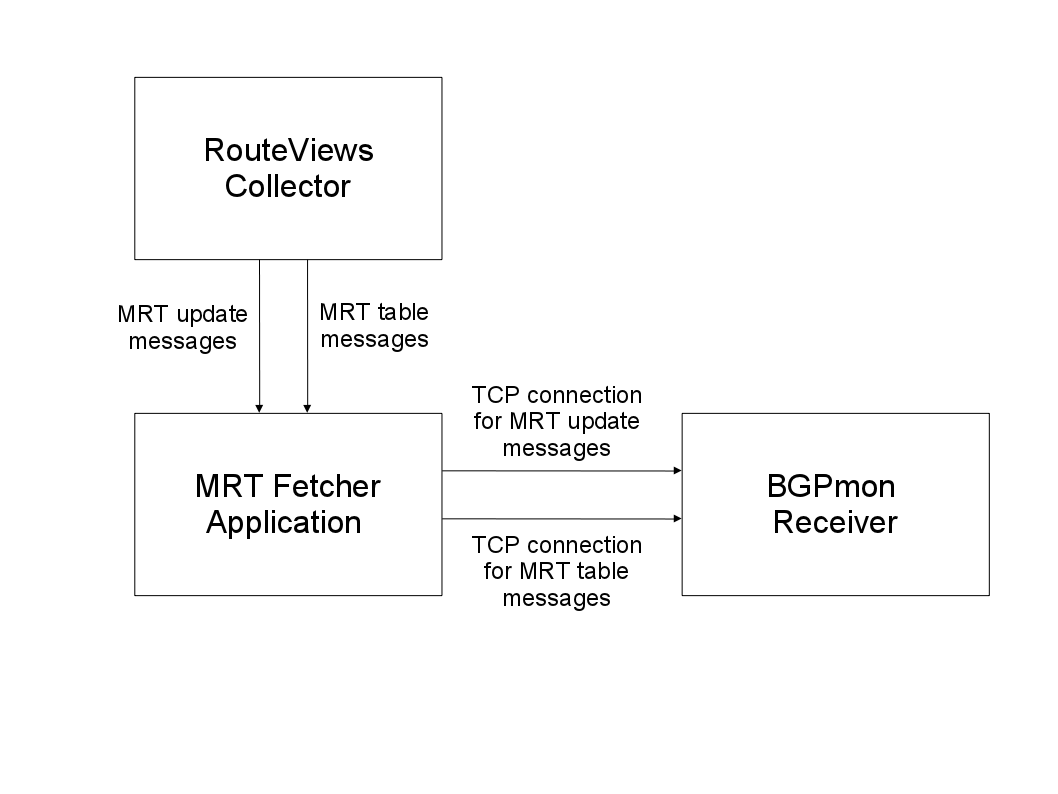
\includegraphics[scale=0.30]{figs/mrtfetcher-design.png}
%\caption{An overview of MRT Fetcher application.}
%\label{fetcherdesignfig}
%\end{figure}

%The MRT fetcher application is designed to run in \emph{collector mode}.  The MRT fetcher %application is designed to send MRT data from the existing routing collectors. Figure %\ref{fetcherdesignfig} shows the MRT fetcher design.  It shows inputs and outputs of the system.  
%The MRT fetcher uses the RouteViews collector to as source of the MRT data. The RouteViews %collector provides the MRT update files and the MRT table files.  
%The MRT fetcher extracts the MRT messages from the MRT update files and the MRT table files. 
% The BGPmon application is receiver that receives MRT messages. The top TCP connection shown in %Figure \ref{fetcherdesignfig} is designed to send MRT update messages from the MRT update file.     %The bottom TCP connection is designed to send MRT table messages from the MRT table file. 

%The MRT feeder creates two TCP connection to BGPmon application. One TCP connection is used to send the MRT table messages. Another TCP connection is designed to  send the MRT update messages. 

%\begin{figure}
%\centering
%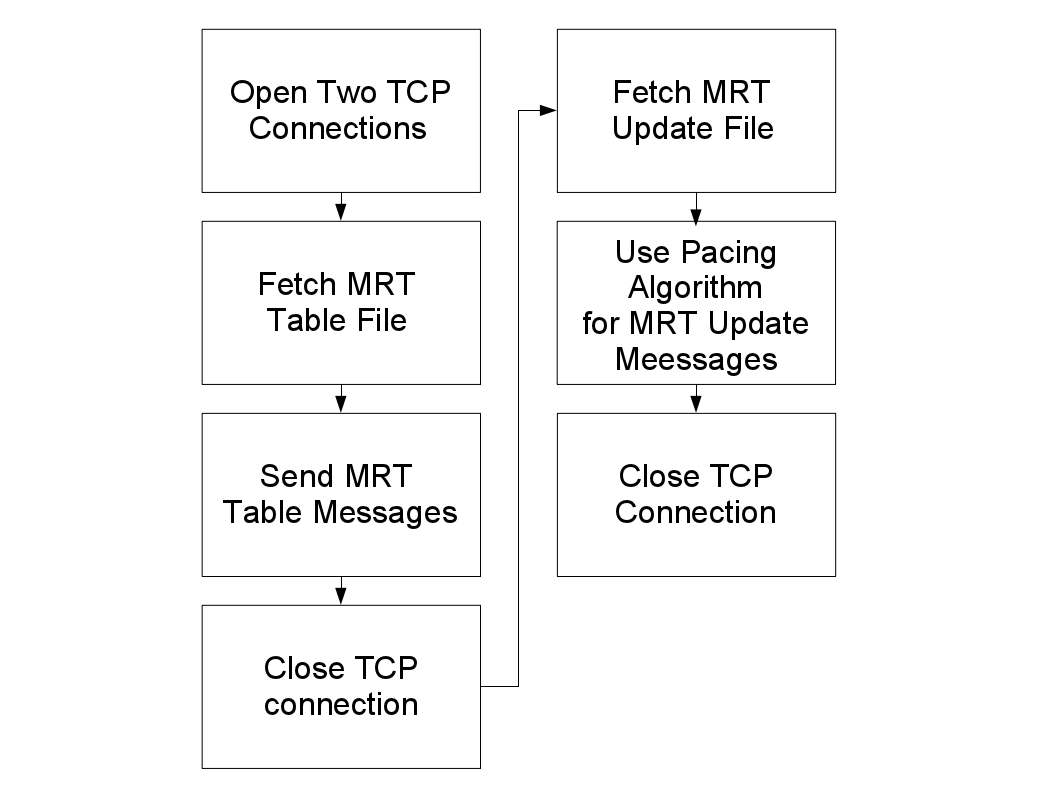
\includegraphics[scale=0.30]{figs/mrtfetcher-flow.png}
%\caption{MRT Fetcher Data Flow Overview.}
%\label{fetcherflowfig}
%\end{figure}

%Figure \ref{fetcherflowfig} shows the data flow in MRT feeder. There are few simple components that are used in the MRT Feeder. First, MRT fetcher opens two  TCP connections to BGPmon application.  Second, the MRT fetcher downloads an archived MRT table file from RouteViews collector. The MRT fetcher extracts the archive and sends the MRT table file to  BGPmon application.  Once the data is sent out, the MRT fetcher closes the TCP connection.  Further, the MRT fetcher downloads an archived MRT update file. It extracts the MRT file and uses \emph{timeframing} algorithm to send MRT messages to BGPmon application.  The \emph{Timeframing} algorithm is discussed in details  in Section \ref{sec:timeframing}. Once the MRT fetcher reaches the end of the MRT update file, it closes TCP connection to BGPmon receiver.   

%The MRT fetcher sends MRT data based on the specified  start time and end time.   The MRT fetcher rounds down the start time and the end time to get the most recent MRT table messages and MRT update messages.   For example,  the user may specify the start time of \emph{Sept 20th, 2011, 9:45 am}  in the MRT fetcher. The RouteViews collector provides the MRT snapshot with MRT table messages every two hours. The MRT fetcher will use \emph{Sept 20th, 2011,  8:00am} MRT snapshot  as the most recent MRT table data source.   Once the MRT table messages are sent, the MRT fetcher will close the first TCP connection and start sending sequence of MRT update messages over the second TCP connection. The RouteViews collector provides the MRT update files with MRT update messages every 15 minutes. The MRT fetcher rounds down the start time and end time for MRT update files. For example, if  the user of the MRT fetcher, assigns a time of \emph{Sept 20th, 2011, 9:45 am} as the start time and \emph{Sept 20th, 2011, 10:10am} as the end time, MRT fetcher will send two MRT update files, first at the time of \emph{Sept 20th, 2011,  9:45 am} and  second at the time of \emph{Sept 20th, 2011, 10:00 am}. 

%The MRT fetcher application is similar to the  MRT feeder application, but it designed to send the MRT files from existing routing collectors. 

  
%The MRT fetcher has following running options:

%\begin{verbatim}
%$ mrtfetcher [-q] [-u] [-c collector] [-s starttime] 
%        [-e endtime]  [-d hostname]
%\end{verbatim}
%where
%\begin{itemize}
%\item{\emph{-q} option instructs MRT fetcher to keep TCP connection when the MRT fetcher sent all %MRT messages.}
%\item{\emph{-u} option instructs MRT fetcher to send the MRT update messages only. This option %skips fetching MRT table files.}
%\item{\emph{-c collector} is used to specify one the RouteView collectors.}
%\item{\emph{-s starttime} is unix timestamp that is used to start sending MRT data.}
%\item{\emph{-e endtime} is unix timestamp that is used to end sending MRT data.}
%\item{\emph{-d hostname} is a name of the host with BGPmon receiver.}
%\end{itemize}


%The MRT fetcher sends two types of MRT data: MRT table files and MRT update files.  The MRT fetcher uses RouteViews collector to fetch the MRT table and the MRT update files. The MRT fetcher creates two TCP connection to BGPmon.  
 
  

% The MRT fetcher is designed to use   \emph{timeframing} algorithm to play MRT messages at the right speed.  The MRT fetcher uses MRT feeder's \emph{timeframing} algorithm described in Section \ref{sec:mrtfeederdesign}.  The MRT fetcher uses \emph{timeframing} for the MRT update messages that originated  between the specified start time and the end time.  For instance,  the tester specified start time of \emph{Sept 20th, 2011, 9:45 am} and end time of \emph{Sept 20th, 2011, 10:10 am}.  First, the MRT fetcher will round down the start time and use the nearest MRT table snapshot at the  \emph{Sept 20, 2011, 8:00 am}.  Second, the MRT fetcher will start sending MRT update files from   \emph{Sept 20th, 2011, 8:00 am} to \emph{Sept 20th, 2011, 9:45 am}. Those MRT update messages will be processed without the timeframing. The MRT update messages from \emph{Sept 20th, 2011, 9:45 am} to \emph{Sept 20th, 2011, 10:10 am} will have the \emph{timeframing} and they will be played at the right speed to the BGPmon receiver.



%The MRT fetcher and MRT feeder have common functionality. For example, both applications are designed to send MRT files to BGPmon receiver. Both application use \emph{timeframing} to play MRT messages at the right speed.  In order avoid  duplicate code, MRT fetcher uses the library functions of MRT feeder. For example, MRT fetcher uses a function from MRT feeder that sends MRT messages over the TCP connection.  


%sends to use already collected MRT files.  The  MRT fetcher use MRT files from the RouteViews archive.  The RouteViews archive provides two types of MRT files: MRT table files and MRT update files. The MRT fetched use MRT table and MRT update files to inject MRT messages into BGPmon instance.  



%MRT fetcher application sends MRT messages in

%* How the Fetcher design looks like?
%* How does it work?  2 tcp connections? 
%* What are the inputs?  What are the outputs? 
%* Options to run ?
%* Timeframing? 
%* How to send updates only? Should be an option. 


%\subsubsection{MRT Analyzer Design Overview}
%\label{sec:mrtfetcherdesign}

%MRT analyzer is a tool that designed to help  in debugging. MRT analyzer outputs a number of %statistics about the peers in MRT file. 
  
%The MRT analyzer has following running options:


%\begin{verbatim}
%$ mrtanalyzer [-c filename] [-d directory]
%\end{verbatim}
%  where:  
%  \begin{itemize}
%  \item{\emph{-c filename} is MRT file. }
%  \item{\emph{-d directoy} is the output directory. MRT analyzer produce output in specified %directory.}
%  \end{itemize}

%The MRT analyzer takes an MRT file as input.   The MRT analyzer uses \emph{bgpdump} tool to extract MRT messages.  The MRT analyzer takes the output from \emph{bgpdump} tool and finds the list of unique peers. The list of peers is stored as \emph{peerlist.txt} in output directory.  For each peer, the MRT analyzer constructs the routing table.  For example, at the time \emph{Sept 22th, 2011, 10:15:00 am} peer \emph{12.0.1.63} received two announce messages with   \emph{11.0.0.0/8} and \emph{13.0.0.0/8} network prefixes. Later, at \emph{Sept 22th, 2011, 10:15:30 am} there was a withdrawn message that removes the \emph{11.0.0.0/8} network prefix. MRT analyzer analyses the list of announced and withdrawn network prefixes  and leave the most recent routes in  table. In example above, \emph{12.0.1.63} peer would have \emph{13.0.0.0/8} prefix in \emph{12.0.1.63\_table.txt} file in output directory. 
 


